\begin{abstract}
   This work introduces a novel framework for 3D pose estimation and motion synthesis in combat sports, leveraging a sparse multi-camera setup and computer vision-based tracking. The approach employs epipolar constraints and long-term video object segmentation to ensure consistent tracking across views and high-quality 2D pose extraction using a top-down transformer-based approach. The 3D pose estimation is achieved through weighted triangulation, spline fitting, and extended Kalman filtering, enhanced by kinematic optimization and physics-based trajectory refinement. Our dataset comprises four hours of two-person boxing sessions, capturing precise skeleton motions and synthetic VR sensor data. We are currently developing a generative motion diffusion model for interactions between two individuals. This model introduces a novel architecture that utilizes a seq2seq model to generate responsive and meaningful motions for a sequence of VR sensor input data.

To ensure physical plausibility, we propose latent physics optimization for the generated motions. This optimization aims to refine contacts and movements, ensuring they adhere to realistic physical constraints.

\begin{CCSXML}
<ccs2012>
<concept>
<concept_id>10010147.10010371.10010352.10010381</concept_id>
<concept_desc>Computing methodologies~Pose Estimation</concept_desc>
<concept_significance>300</concept_significance>
</concept>
<concept>
<concept_id>10010147.10010371.10010352.10010382</concept_id>
<concept_desc>Computing methodologies~Motion synthesis</concept_desc>
<concept_significance>300</concept_significance>
</concept>
</ccs2012>
\end{CCSXML}

\ccsdesc[300]{Computing methodologies~Pose Estimation}
\ccsdesc[300]{Computing methodologies~Motion synthesis}


\printccsdesc   
\end{abstract}  
%-------------------------------------------------------------------------
\section{Introduction}

Combat sports present significant challenges for motion capture due to numerous close-proximity interactions and frequently crowded backgrounds. 
Optical markers tracking is precise in a laboratory setting, yet are impractical for combat sports due to the highly dynamic motions and frequent collisions that lead to calibration issues with markers. Inertial measurement unit (IMU) based solutions suffer from global positional drift, affecting inter-athlete distances. Monocular vision-based approaches leave athletes unencumbered by tracking equipment, but they lack precision due to insufficient visual data arising from frequent occlusions. Issues due to occlusion can however be mitigated by incorporating camera data from multiple viewpoints, an idea that we built on in our tracking pipeline.

We propose a multi-stage multi-view tracking pipeline that is capable of reconstructing high-quality 3D motion of athletes participating in combat sports, such as boxing. Our approach fuses 2D keypoints from multiple camera views by a kinematic optimization.  This is followed by a physics-based trajectory optimization utilizing model predictive control to eliminate non-physical artifacts. 

\section{Pose Estimation}
\textbf{Epipolar Geometry:} Epipolar constraints use geometric lines (epipolar lines) to associate corresponding points across different camera views. These constraints are defined by the fundamental matrix ($\mathbf{F}$), facilitating efficient matching by restricting search space along these lines.

\textbf{Tracking 2D and 3D Data:} Using epipolar constraints and long-term video object segmentation Triangulation computes 3D positions from 2D keypoints across multiple cameras using their projection matrices. It solves a linear system to determine 3D coordinates, weighting contributions based on 2D keypoints’ confidence. Techniques like SVD solve this system, with subsequent filtering and smoothing ensuring robust 3D reconstructions, even in the presence of noise and outliers.

\textbf{Kinematics Optimization:} The kinematics optimization methodology discussed focuses on refining the pose estimation of athletes using a hybrid approach of 2D and 3D keypoint data. Employing the SMPL model, the optimization aims to minimize the disparity between model joints and observed data while ensuring temporal coherence and natural movement. This is achieved through a comprehensive objective function that includes terms for smoothness, similarity to human motion priors, and alignment with both 2D re-projection evidence and triangulated 3D keypoints.

Initially, the optimization initializes shape parameters ($\beta \in \mathbb{R}^{10}$) of the SMPL model based on 3D keypoints obtained through triangulation. Subsequently, it iteratively adjusts these parameters alongside pose parameters ($\theta \in \mathbb{R}^{72}$) to refine the pose estimation. The process integrates a Limited-memory Broyden–Fletcher–Goldfarb–Shanno (LBFGS) optimizer, configured with specific parameters for efficient minimization of the objective function.

Key components of the objective function include:

\begin{itemize}
    \item \textbf{2D Re-projection Loss} ($\mathrm{L}_\text{2D}$): Aligns 3D joints with 2D joints across multiple camera views, emphasizing joints with high-confidence detections using a robust error function.
    \item \textbf{3D Alignment Loss} ($\mathrm{L}_\text{3D}$): Computes the Euclidean distance between predicted 3D joint positions and triangulated 3D keypoints, weighted by their confidence scores.
    \item \textbf{Smoothness Loss} ($\mathrm{L}_\text{smooth}$): Promotes consistency in pose transitions over time frames and vertices of the posed mesh.
    \item \textbf{Prior Losses} ($\mathrm{L}_{\text{GMM}}$, $\mathrm{L}_{\text{Vposer}}$): Introduces Gaussian Mixture Model (GMM) and Vposer priors to penalize unnatural poses, guiding the optimization towards more realistic and fluid motion.
\end{itemize}

Through experimental validation, the inclusion of these priors has proven effective in reducing limb jitter and enhancing the overall naturalness of the optimized poses. This comprehensive approach ensures accurate and lifelike pose estimation suitable for applications in sports biomechanics and animation.

\begin{figure}[htbp]
  \centering

  \documentclass{standalone}
\usepackage{tikz}
\usepackage{amsmath}
\usepackage[T1]{fontenc}
\tikzset{
    process/.style={draw, rectangle, rounded corners, fill=yellow!20, minimum width=1cm, auto, on grid, minimum height=1cm, align=center},
    process4/.style={draw, font=\fontsize{8}{9.6}\selectfont, rectangle, rounded corners, fill=yellow!20, text width=3cm, auto, on grid, align=center},
    decision/.style={draw, font=\fontsize{8}{9.6}\selectfont, rectangle, rounded corners, fill=red!20, text width=3cm, minimum height=1cm, auto, on grid, align=center},
    process2/.style={draw, font=\fontsize{8}{9.6}\selectfont, rectangle, rounded corners, fill=cyan!20, text width=4cm, auto, on grid, align=center},
    process3/.style={draw, font=\fontsize{8}{9.6}\selectfont, rectangle, text width=4cm, rounded corners, fill=cyan!20, rotate=-90, auto, on grid, align=center},
    vecArrow/.style={thick, decoration={markings,mark=at position 1 with {\arrow[semithick]{open triangle 60}}},
        double distance=1.4pt, shorten >= 5.5pt,
        preaction = {decorate},
        postaction = {draw,line width=1.4pt, white,shorten >= 4.5pt}},
    vecArrow1/.style={thick, decoration={markings,mark=at position 0.9 with {}},
        double distance=1.4pt, shorten >= 5.5pt,
        preaction = {decorate},
        postaction = {draw,line width=1.4pt, white,shorten >= 4.5pt}},
    innerWhite/.style={semithick, white,line width=1.4pt, shorten >= 4.5pt},
}

\usetikzlibrary{arrows, decorations.markings, arrows.meta,positioning,shadows,shapes.geometric,automata,positioning,fit,arrows.meta,calc,bending}


\usepackage{graphicx} % for including images

\usepackage{overpic} % for overlaying text on images

\begin{document}
\resizebox{0.7\textwidth}{!}{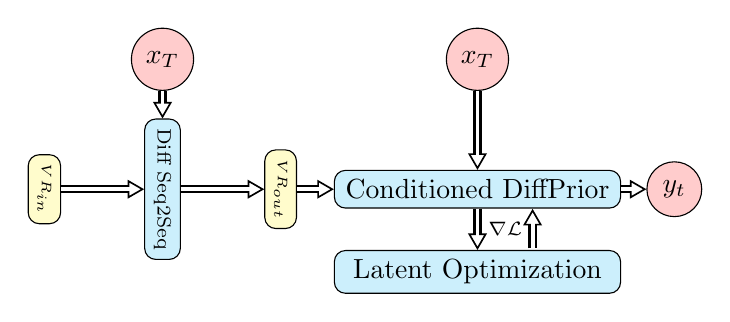
\begin{tikzpicture}[node distance=2cm]
\tikzstyle{process}=[draw, font=\fontsize{5}{4.8}\selectfont, rectangle, rounded corners, fill=yellow!20, minimum width=1cm, auto, on grid, minimum height=1cm, align=center]

\tikzstyle{decision}=[draw, font=\small, rectangle, rounded corners, fill=red!20, text width=3cm, auto, on grid, align=center]
\tikzstyle{process2}=[draw, font=\fontsize{9}{4.8}, rectangle, rounded corners, fill=cyan!20, text width=3.4cm, auto, on grid, align=center]
\tikzstyle{circlenode}=[draw, circle, fill=red!20, minimum size=1mm]
\tikzstyle{process3}=[draw, font=\fontsize{7}{4.8}\selectfont, rectangle, rounded corners, fill=cyan!20, rotate=-90, auto, on grid, align=center]
\tikzstyle{process4}=[draw, font=\fontsize{5}{4.8}\selectfont, rectangle, rounded corners, fill=yellow!20, rotate=-90, auto, on grid, align=center]
\tikzstyle{vecArrow} = [thick, decoration={markings, mark=at position 1 with {\arrow[semithick]{open triangle 60}}}, double distance=1.4pt, shorten >= 5.5pt, preaction = {decorate}, postaction = {draw, line width=1.4pt, white, shorten >= 4.5pt}]
\tikzstyle{vecArrow1} = [thick, decoration={markings, mark=at position 0.9 with {}}, double distance=1.4pt, shorten >= 5.5pt, preaction = {decorate}, postaction = {draw, line width=1.4pt, white, shorten >= 4.5pt}]
\tikzstyle{innerWhite} = [semithick, white, line width=1.4pt, shorten >= 4.5pt]

\node[process4] (input) at (-4.5, -0.35) {${VR}_{in}$};
\node[process3] (seq2seq) at (-3, -0.35) {Diff Seq2Seq};
\draw[vecArrow] (input) -- (seq2seq);
\node[process4] (output) at (-1.5, -0.35) {${VR}_{out}$};
\draw[vecArrow] (seq2seq) -- (output);
\node[process2] (prior) at (1, -0.35) {Conditioned DiffPrior};
\node[circlenode] (yt) at (3.5, -0.35){$y_t$};
\node[circlenode] (xt) at (1, 1.3){$x_T$};
\node[circlenode] (xt1) at (-3, 1.3){$x_T$};
\draw[vecArrow] (prior) -- (yt);
\draw[vecArrow] (xt1) -- (seq2seq);
\draw[vecArrow] (xt) -- (prior);

\draw[vecArrow] (output) -- (prior);
\node[process2] (optimization) at (1, -1.4) {Latent Optimization};
\draw[vecArrow] (prior) -- (optimization);
\draw[vecArrow] (1.7, -1.1) tonode[anchor=east] {\scriptsize $\nabla \mathcal{L}$} (1.7, -0.6);


\end{tikzpicture}}
\end{document}

  \caption{\label{fig:condtion-diffusion}
           The condition for the seq2seq model contains the VR sensor information of the player and the output is the corresponding VR sensor input for the opponent at each sequence. The conditional diffusion prior is conditioned on the opponent synthetic information and produces the whole body pose for the opponent. The optimization in loop make sure the output motion has the desired trajectories based on a loss function.}
\end{figure}

Figure~\ref{fig:condtion-diffusion} which need the full textwidth can be typeset as Figure.

%-------------------------------------------------------------------------
\textbf{Dynamics Optimization:} In the described study, a two-stage optimization approach is employed to enhance the accuracy and quality of motion tracking for athletes. The initial stage focuses on kinematic optimization, which estimates full-body poses but often introduces high-frequency artifacts known as jitter. To mitigate this, a second stage employs dynamics optimization using a physics-based humanoid model. This model, derived from joint positions and landmarks of an SMPL mesh, creates an articulated rigid-body structure with capsule collision geometry, featuring 56 joint-angle degrees of freedom and a 6 degree of freedom root joint.

The dynamics optimization stage aims to refine motion trajectories by considering joint torques and biomechanical constraints within a physical environment. It computes joint torques using an iterative Linear Quadratic Regulator (iLQR) algorithm, which optimizes control inputs to smooth and stabilize motion trajectories while adhering to physical realism. This approach accounts for contact forces and body dynamics, enhancing the overall quality and naturalness of the generated motions.

Furthermore, trajectory optimization in this framework minimizes a weighted sum of regularization terms and loss functions, which include penalties for velocity and control values. By iteratively refining control trajectories over short time horizons, the method achieves improved alignment with desired motion characteristics derived from the kinematic stage outputs. Overall, this integrated approach ensures robust and realistic motion tracking suitable for applications in sports biomechanics and animation.

\section{Motion Synthesis}
%---------------------------------------------------------------------
\textbf{Interaction Diffusion Model:}
 
A novel application of sequence-to-sequence (seq2seq) models in virtual reality involves generating responsive opponent motions based on sparse VR input data. In this context, the seq2seq model serves as a pivotal tool for translating sparse signals captured from VR sensors into realistic and dynamic movements for virtual opponents. Trained on a specialized multi-person boxing dataset, the model learns to map the sparse input, which could include data from wearable IMUs or HMDs, into coherent sequences of actions that simulate human-like behavior during a boxing match. By leveraging the dataset’s diverse scenarios and real-world motion variations, the seq2seq model not only predicts the opponent’s reactions but also adapts to different player actions, enhancing the realism and engagement of VR gaming experiences. This approach marks a significant advancement in interactive VR applications by bridging the gap between sparse sensor data and immersive virtual interactions, thereby enriching the user experience through responsive and lifelike virtual opponents.
%---------------------------------------------------------------------
\textbf{Conditioned Diffprior:}
The application of conditional diffusion models, specifically tailored for full-body motion synthesis from sparse IMU tracking signals, represents a breakthrough in virtual reality (VR) body tracking. This approach overcomes the inherent challenges of accurately predicting smooth and realistic full-body motions with minimal input data. By leveraging a lightweight MLP architecture and employing a block-wise injection scheme for embedding time step information, the conditional diffusion model effectively reduces artifacts like jittering and enhances robustness against signal loss. These advancements are underscored by its superior performance on benchmarks like the AMASS dataset, setting new standards in motion prediction methods.

In parallel, the conditional diffusion model paradigm also finds application in frameworks designed for real-time human motion tracking in VR environments. This innovative approach integrates scalable 3DOF IMUs with head-mounted displays (HMDs), offering a flexible solution that balances tracking accuracy with user-friendliness across various VR setups. Central to its efficacy is a lightweight temporal-spatial feature learning (TSFL) network, combining LSTM for temporal feature capture and Transformer for spatial correlation learning. This hybrid architecture optimizes computational efficiency while maintaining high accuracy in estimating full-body poses, making it suitable for immersive VR experiences demanding fluid and responsive interactions.

%---------------------------------------------------------------------
\textbf{Latent Optimization:}

Optimize noisy motion inputs directly in the latent space of the diffusion model. By treating motion denoising as a black box and iteratively adjusts the diffusion noise vector using gradients computed through an ODE solver, ensuring the output motion meets user-defined criteria. This approach avoids the need for fine-tuning models for specific tasks, demonstrating superior performance in motion editing, preservation, and task fulfillment compared to existing methods.